\begin{ZhChapter}

\chapter{若標題太長,則可以分成兩行排列的形式撰寫}

\section{名詞定義(小標)}

定義定義定義定義定義定義\cite{112TIT00392032},定義定義定義定義,定義定義定義定義定義定義定義定義定義定義,定義定義。

\begin{table*}[htbp]
    \centering
    \caption{表格範例標題} \label{tab: complexity}
    \makebox[\linewidth][c]{
    \renewcommand\arraystretch{1.2}{
        \begin{tabular}{| l | c  c  c  c |}
        \hline
        Protocol & $P$ & $CS_1$ & $CS_2$ & $RG$ \\
        \hline
        MSSMul & $O(1)$, $O(1)$, N/A & $O(n-t)$, $O(n)$, $O(1)$ & $O(n-t)$, $O(n)$, N/A & $O(1)$, $O(n)$, $O(n)$ \\
        SC & $O(1)$, $O(1)$, N/A & $O(n-t)$, $O(n)$, $O(1)$ & $O(n-t)$, $O(n)$, N/A & $O(1)$, $O(n)$, $O(n)$ \\
        \hline 
        \end {tabular}
    }}
\end {table*}

\section{模型說明(小標)}

說明說明說明說明,說明說明說明說明說明說明說明說明說明說明說明說明,說明說明說明說明說明說明說明說明。

\begin{figure*}[htbp]
    \centering
    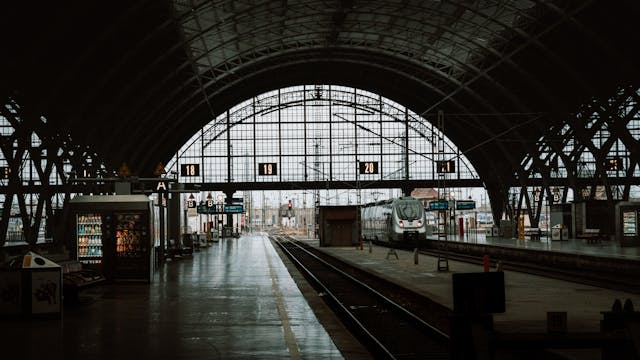
\includegraphics[width = 0.5\textwidth]{image/image.jpeg}
    \caption{Cool train station}
    \label{fig: image}
\end{figure*}

\end{ZhChapter}